\documentclass[handout,a4paper,slidestop,xcolor=pst,blue]{beamer}

\input{slidesHeader.tex}
\usepackage{listings}

\definecolor{pblue}{rgb}{0.13,0.13,1}
\definecolor{pgreen}{rgb}{0,0.5,0}
\definecolor{pred}{rgb}{0.9,0,0}
\definecolor{pgrey}{rgb}{0.46,0.45,0.48}

\lstset{language=Java,
  showspaces=false,
  showtabs=false,
  breaklines=true,
  showstringspaces=false,
  breakatwhitespace=true,
  commentstyle=\color{pgreen},
  keywordstyle=\color{pblue},
  stringstyle=\color{pred},
  basicstyle=\ttfamily,
  keywordsprefix={@}
}


\newcommand{\ann}[1]{\color{blue}\texttt{#1}\color{black}}

\title[JPA + Spring Data]{Capa de Servicios - Spring Rest Controllers}

\author[P. S{\'a}nchez]{\alert{Pablo S{\'a}nchez}}

\institute[IIE]{
		   Dpto. Ingenier{\'i}a Inform{\'a}tica y Electr{\'o}nica \\
		   Universidad de Cantabria \\
		   Santander (Cantabria, Espa{\~n}a) \\
		   \texttt{p.sanchez@unican.es}
}

\date{}

\begin{document}

\begin{frame}[c]
	\titlepage
	\begin{columns}
		\column{0.50\linewidth}
			\centering
    		\includegraphics[width=.28\textwidth,keepaspectratio=true]{images/istr.eps}
		\column{0.50\linewidth}
			\centering
			\includegraphics[width=.25\textwidth,keepaspectratio=true]{images/uc.eps}
	\end{columns}
\end{frame}

\begin{frame}[c]
    \frametitle{\alert{Advertencia}}
    \begin{center}
        Todo el material contenido en este documento no constituye en modo alguno una obra de referencia o apuntes oficiales mediante el cual se puedan preparar las pruebas evaluables necesarias para superar la asignatura. \ \\
        \ \\
        Este documento contiene exclusivamente una serie de diapositivas cuyo objetivo es servir de complemento visual a las actividades realizadas en el aula para la transmisi{\'o}n del contenido sobre el cual versar{\'a}n las mencionadas pruebas evaluables.  \ \\
        \ \\
        Dicho de forma m{\'a}s clara, \alert{estas transparencias no son apuntes y su objetivo no es servir para que el alumno pueda preparar la asignatura.}
    \end{center}
\end{frame}

\section{Introducción}

\begin{frame}[c]
    \frametitle{Objetivos del Tema}
    \begin{enumerate}[<+->]
         \item Ser capaz de crear controladores REST utilizando \emph{Spring}.
         \item Ser capaz de especificar cómo serializar POJOs usando \emph{Jackson}.
         \item Ser capaz de especificar transaccionalidad usando \emph{Spring}.
    \end{enumerate}
\end{frame}

%\begin{frame}[c]
%    \frametitle{Bibliografía}
%    \begin{thebibliography}{1}
%
%        \bibitem[Spring, 2019]{Spring2019}
%        \em {Spring Reference Documentation}.
%        \newblock{\url{https://goo.gl/AzsbtY}}
%
%    \end{thebibliography}
%\end{frame}

\begin{frame}[c]
    \frametitle{Arquitectura MVC}
    \begin{center}
        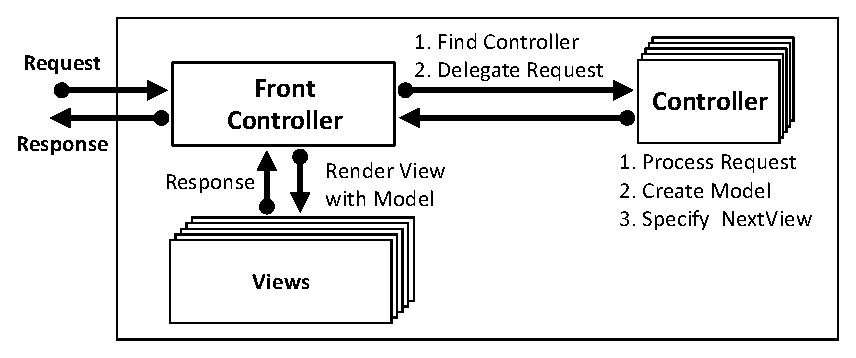
\includegraphics[width=\linewidth,keepaspectratio=true]{images/mvc/mvc00.eps}
    \end{center}
\end{frame}

\section{Spring Rest Controllers}

\begin{frame}[c]
    \frametitle{Anotaciones Rest}
    \begin{tabular}{lp{0.70\linewidth}}
        \ann{@RestController} &  La clase contendrá controladores REST. \\
        \ann{@RequestMapping} &  URI raíz asociada a un \texttt{RestController}. \\
        \ann{@GetMapping}     &  Controlador GET (de la URI correspondiente).  \\
        \ann{@PostMapping}    &  Controlador POST (de la URI correspondiente). \\
        \ann{@PutMapping}     &  Controlador PUT (de la URI correspondiente). \\
        \ann{@DeleteMapping}  &  Controlador DELETE (de la URI correspondiente). \\
        \ann{@PathVariable}   &  El parámetro se extrae de una variable de la URI. \\
        \ann{@RequestParam}   &  Parámetros de la petición HTTP. \\
        \ann{@RequestBody}    &  Parámetro enviado en el cuerpo de la petición \\
    \end{tabular}
\end{frame}

%\begin{frame}[c]
%    \frametitle{Respuestas Http}
%    \begin{listing}
%         ResponseEntity<T>  & \\
%   \end{tabular}
%\end{frame}

\section{Jackson}

\begin{frame}[c]
    \frametitle{Anotaciones Jackson}
    %% Se mapea todo aquello que tenga getter.
    \begin{tabular}{lp{0.70\linewidth}}
        \ann{@JsonAutoDetect} & \\
        \ann{@JsonProperty("codigo")} & \\
        \ann{@JsonIgnore}        &  \\
        \ann{@JsonManagedReference} &  \\
        \ann{@JsonBackReference} &  \\
        \ann{@JsonUnwrapped} & \\
        \ann{@JsonValue} & \\
    \end{tabular}
\end{frame}

\begin{frame}[c]
    \frametitle{Vistas Jackson}
    %% Se mapea todo aquello que tenga getter.
    \begin{tabular}{lp{0.70\linewidth}}
        \ann{@JsonIgnore}        &  \\
        \ann{@JsonManagedReference} &  \\
        \ann{@JsonBackReference} &  \\
        \ann{@JsonUnwrapped} & \\
    \end{tabular}
\end{frame}

\section{Soporte para Transacciones}


\section{Sumario}

\begin{frame}[c]
    \frametitle{¿Qué tengo que saber de todo ésto?}
    \begin{enumerate}[<+->]
        \item Ser capaz de utilizar anotaciones \emph{Spring MVC} para implementar controladores Rest.
        \item Ser capaz de utilizar anotaciones \emph{Jackson} para serializar POJOs a JSON.
        \item Comprender el funcionamiento del \emph{Entity Manager}.
        \item Ser capaz de utiliza anotaciones para definir transacciones en \emph{Spring}.
    \end{enumerate}
\end{frame}

\end{document}
